% 本文件是示例论文的一部分
% 论文的主文件位于上级目录的 `bachelor.tex` 或 `master.tex`

\chapter{单路口场景智能交通信号调度}
\section{相关工作}
最近,强化学习算法在交通信号控制领域表现出了优异的性能,这些算法将当前道路上的交通状况当作状态,并通过与环境交互学习操控信号的策略。
现有的基于强化学习的交通信号控制方法之间的差异主要体现在以下这三个方面:状态表示、奖励设计以及学习算法。

状态表示是对当前环境的定量描述。一些常见的状态特征包括:
\begin{itemize}
  \item 队列长度(Queue length):队列长度是车道上处于“等待”状态的车辆的数量。对于车辆“等待”状态,有不同的定义。在\inlinecite{wei2018intellilight}中,速度小于$0.1\text{米}/s$的车辆被认为处于等待状态;在\inlinecite{steingrover2005reinforcement,kuyer2008multiagent}中,等待车辆是指没有移动位置的车辆。
  \item 等待时间 (Waiting time):车辆的等待时间定义为车辆处于“等待”状态的时间段。等待期的开始时间的定义可能有所不同,在\inlinecite{van2016coordinated,wei2018intellilight},他们认为等待时间是从车辆移动的最后一个时间戳开始,而\inlinecite{brys2014distributed,pham2013learning}认为等待时间是从车辆进入路网开始的。
  \item 交通流量(Traffic volume):交通流量定义为车道上的车辆数量,等于该车道上处于等待状态的车辆和行驶车辆的总和。
  \item 相位(Phase):将相位信息作为状态特征,首先要将其进行量化,\inlinecite{van2016coordinated,wei2018intellilight}用当前相位在预先定义的信号相位组中的索引值来确定。
\end{itemize}
通常情况下,状态描述会整合多个特征,以获得对交通状况更全面的描述。

在交通信号控制问题中,尽管最终的目标是使所有车辆的行驶时间最小化,但由于一些原因,行驶时间很难直接作为RL的有效奖励。首先,车辆的行驶时间不单单受交通信号的影响,还与其他的因素有关,例如车辆的速度。其次,当交通信号控制器事先不知道车辆的目的地时(现实世界中经常出现这种情况),优化网络中所有车辆的行驶时间变得尤为困难。在这种情况下,只有当网络中的多个交叉路口采取了多项行动时,才能在车辆完成行程后测量车辆的行驶时间。因此,奖励功能通常被定义为下列因素的加权和,这些因素在智能体采取动作后可以被即刻测量出。
\begin{itemize}
  \item 总队列长度:这里队列长度是所有incoming lanes的队列长度之和。\inlinecite{zheng2019diagnosing}证明了最小化队列长度相当于最小化所有车辆的行驶时间。
  \item 吞吐量:吞吐量定义为在最后一个动作后的特定时间间隔内通过交叉路口或离开网络的车辆总数。
  \item 速度:一个典型的奖励是取道路网中所有车辆的平均速度,平均速度越高意味着车辆行驶到目的地的速度越快,时间也就越短。
  \item 信号变化频率:信号改变的频率被定义为在某一时间段内信号改变的次数。直观地说,学到的政策不应该导致闪烁,即频繁地改变交通信号,因为车辆通过交叉口的有效绿色时间可能会减少。
\end{itemize}
\section{已有工作中的不足}
虽然目前已经有不少基于强化学习的智能交通信号控制的研究,但是已有的方法更多的只注重提高通行效率,例如最小化队列长度或者最大化吞吐量,而忽略了公平性问题。事实上,这样的目标会导致学习到一个有偏见的策略。例如可能会出现如\autoref{fig:last-vehicle}所示的"last-vehicle"情况:N-S方向的道路上有源源不断的车辆到达,而E-W方向上是该车流的最后一辆车(Last-Vehicle)。显然,为了最大化通行效率,会优先放行N-S方向上的车流,而E-W车道上的车要等所有的所有的车流通过才能够得到响应,这对Last-Vehicle来说是极其不公平的。

\begin{figure}[t]
  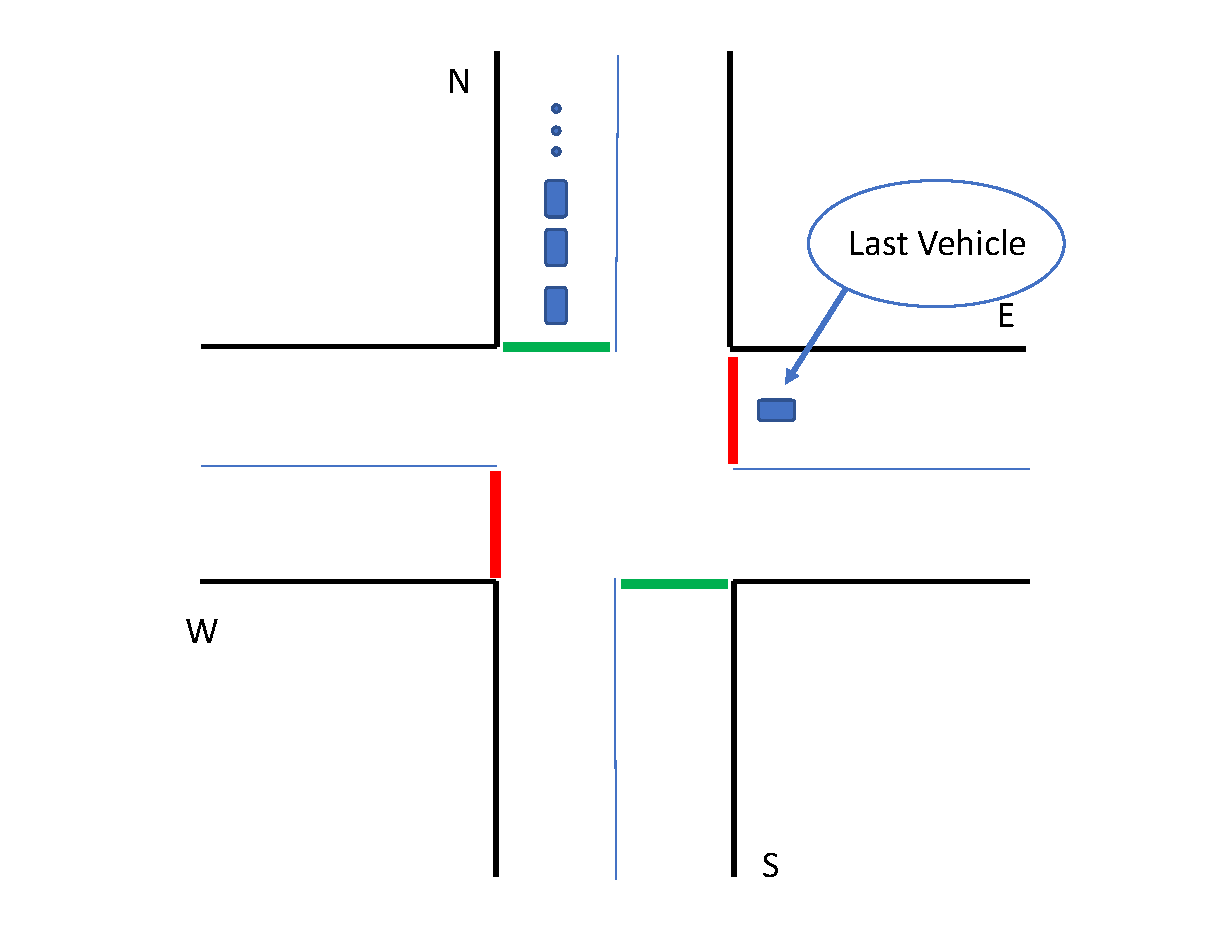
\includegraphics[width=0.9\textwidth]{fig/lastvehicle.pdf}
  \caption{last vehicle}
  \label{fig:last-vehicle}
\end{figure}

\section{改进}
\subsection{目标}
本工作的目的是在提高通行效率(最小化平均通行时间)的同时,希望每条车道能够有尽可能相同的服务延迟(得到放行所需的时间)。
\subsection{智能体设计}
\subsection*{状态表示}
在$t$时刻的状态$S(t)$由以下几个部分组成:
\begin{enumerate}
\item 交通流量:$\boldsymbol{V}(t)=\{V_1(t),V_2(t),\cdots,V_M(t)\}$。其中 $V_i(t)$表示第$i$条进近车道上车的数量。值得注意的是,由于右转不受限于信号灯的特殊性,这里我们不考虑右车道的交通流量。
\item 平均吞吐量:$\boldsymbol{\overline{L}}(t)=\{\overline{L}_1(t),\overline{L}_2(t),\cdots,\overline{L}_M(t)\}$。其中$\overline{L}_i(t)$表示第$i$条进近车道的平均吞吐量。同上,不考虑右车道的平均吞吐量。
\item 信号相位:$\boldsymbol{P}(t)$是当前信号相位的数字化表示,$1$表示绿色,可以通行;$0$表示红色,禁止通行。
\end{enumerate}
所以$S(t)=\{\boldsymbol{V}(t) || \boldsymbol{\overline{L}}(t) || \boldsymbol{P}(t) \}$
\subsection*{动作选择}
在本文中,动作选择机制是每次选择即将转换的信号相位。之后,交通信号灯将转换到这一新的相位并持续$\Delta t$的时间。为了安全起见,我们在两个不同的信号相位之间插入了3秒的黄色信号和2秒的红色信号。如果新选择的相位和当前相位相同,则不插入黄色和红色信号,以确保交通流畅。
\subsection*{奖励函数}
受PFS分配原则的启发,我们设计了一个可以在效率和公平之间提供良好的平衡的奖励函数,如下所示:
\begin{align}
\label{eq:reward}
    r = -\sum_{i=1}^{M} \frac{Q_i(t)}{\overline{L}_i(t) + \delta},
\end{align}
其中$Q_i(t)$ 和 $\overline{L}_i(t)$ 分别是第$i$条进近车道的队列长度和平均吞吐量。在每一次调度后(这里,我们将一次动作选择视作一次调度),$\overline{L}_i(t)$ 按照以下方式进行更新:
\begin{align}
    \overline{L}_i(t) = (1-\frac{1}{W})\overline{L}_i(t-1) + \frac{1}{W}L_i(t),
\end{align}
其中$L_i(t)$是此次调度中车道$i$上得到放行的车的数量,$W$是一个平衡通行效率和公平性的参数。另外,为了避免公式\ref{eq:reward}的分母为0, 我们加上了一个可以忽略不计的正数$\delta$。

\begin{figure}[htb]
  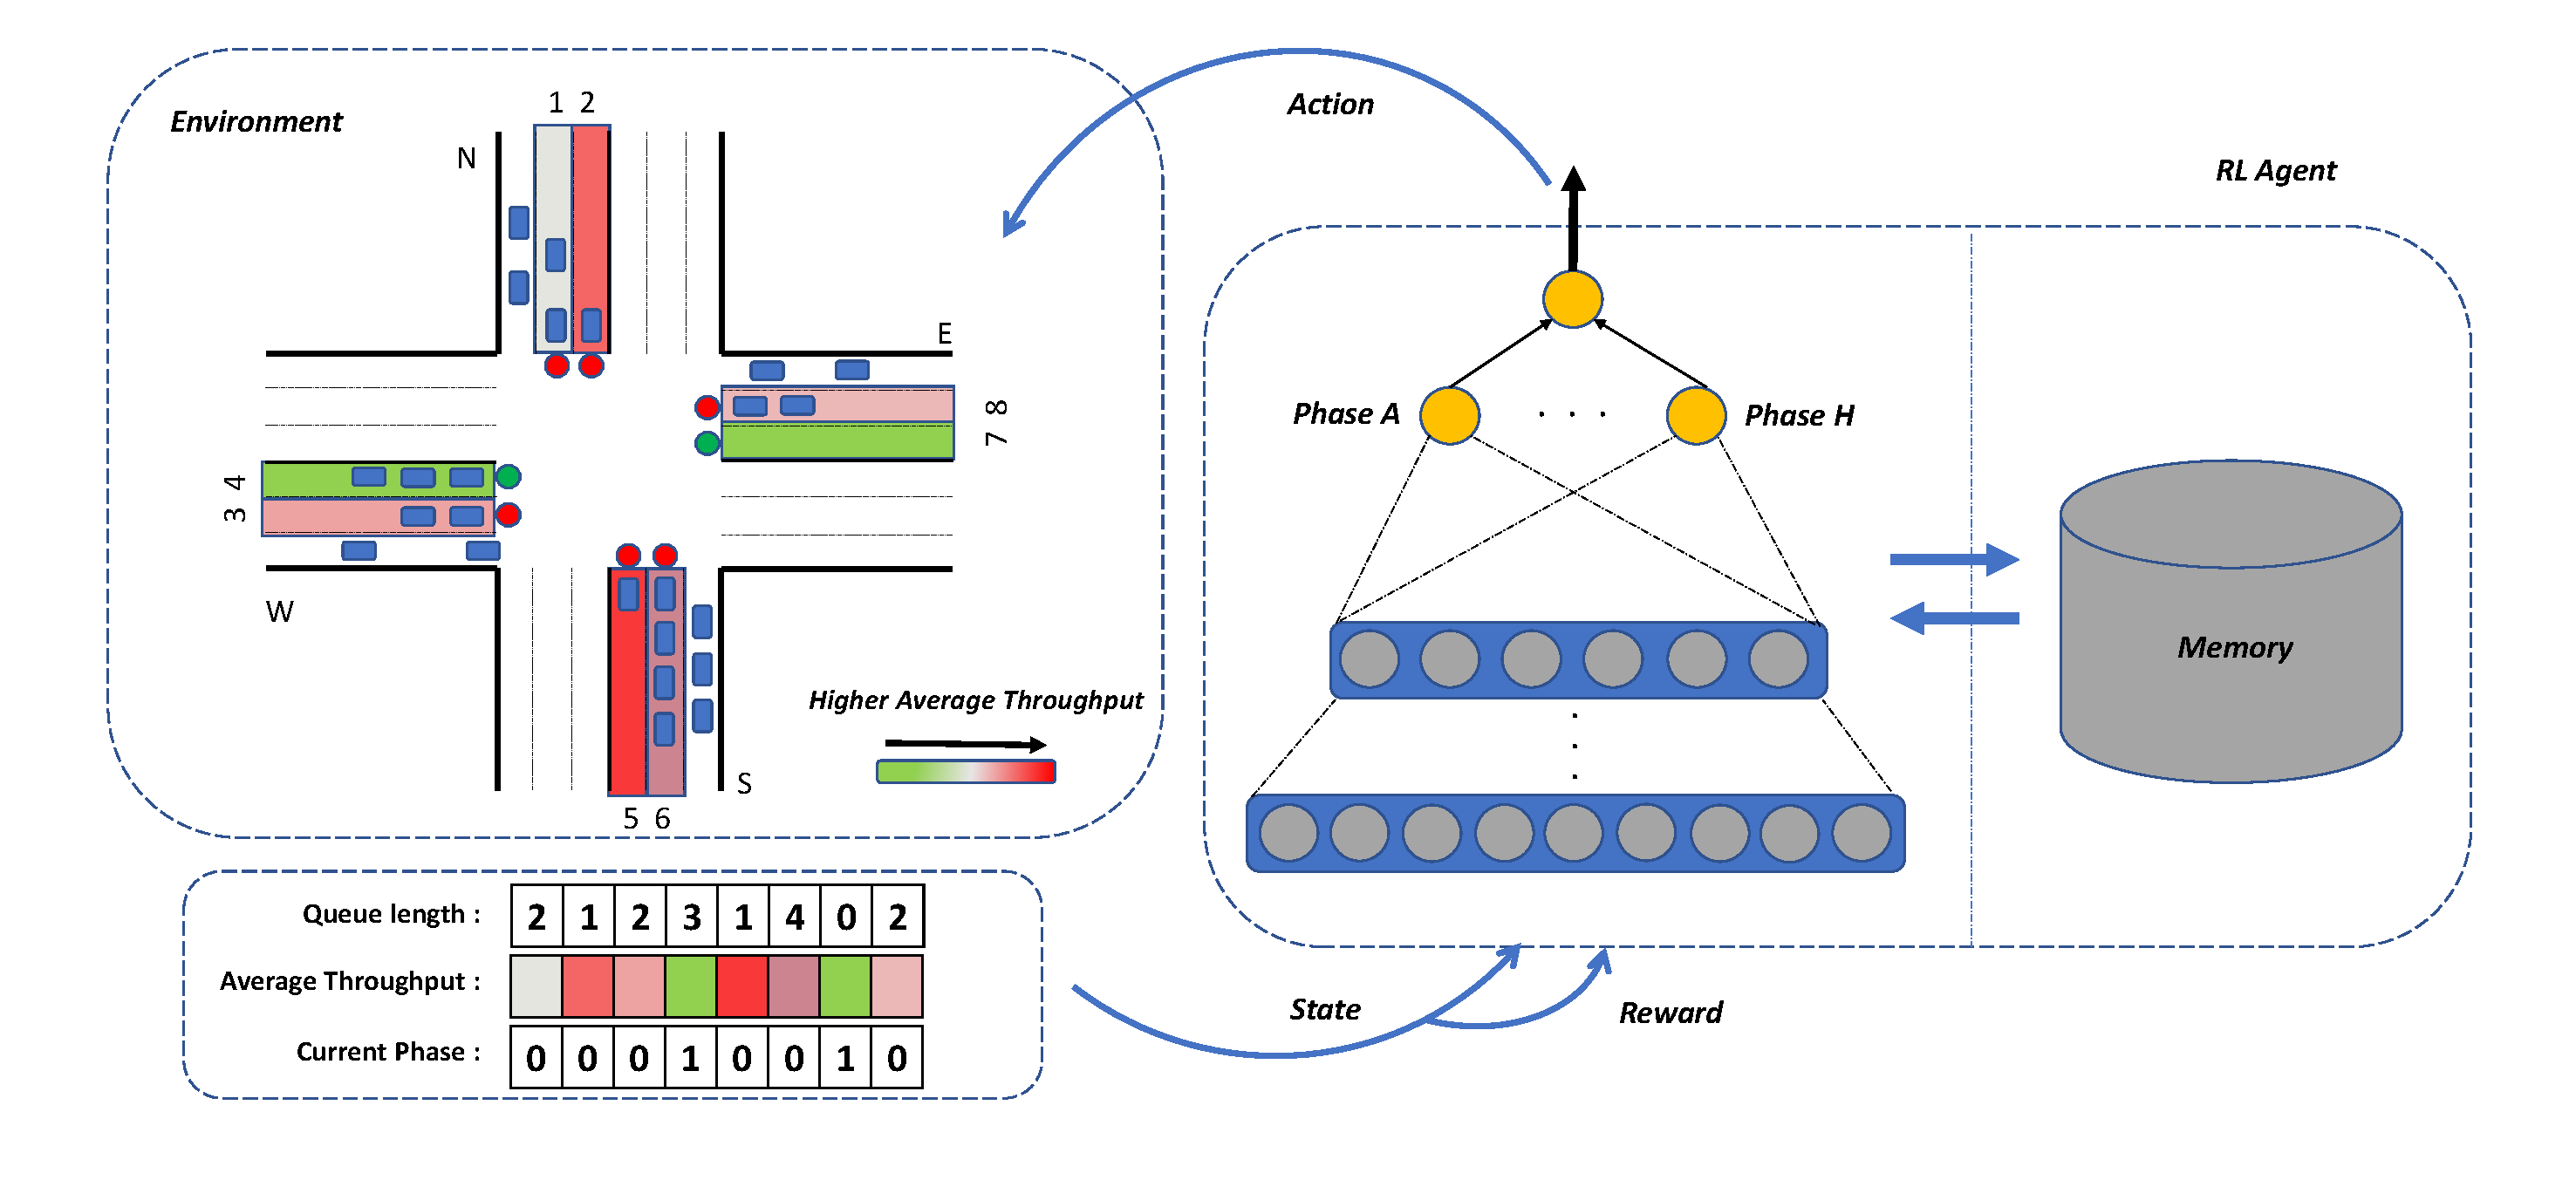
\includegraphics[width=.9\textwidth]{fig/sysmodel.pdf}
  \caption{系统模型}
  \label{fig:system-model}
\end{figure}

\subsection*{模型框架}
如\autoref{fig:system-model}所示,这里我们用DQN作为学习算法,并且采用经验回放\cite{mnih2015human}(experience replay)方法定期提取样本来更新模型,具体算法过程如\autoref{alg:dqn-single}所示。
\begin{breakablealgorithm}
    \caption{基于DQN的交通信号控制训练流程}
    \label{alg:dqn-single}
    \begin{algorithmic}[1] %每行显示行号  
        \Require 
        $E$ : 学习片段数 \newline
        $T$ : 每个学习片段的步数 \newline
        $b$ : 学习经验数 \newline
        $\epsilon$ : 随机选择动作概率 \newline
        $\gamma$ : 折扣因子 \newline
        $\Delta t$ : 信号维持时间
        \For{$episode=1,E$}  
            \State 初始化环境。
            \State 生成车辆。
            \For{$t=1,T$}
                \State 从环境中获取状态观测$s_t$。
                \State 生成一个0到1之间的随机数$rand$。
                \If{ $rand < \epsilon$}
                    \State 从动作空间中随机采样一个动作$a_t$。
                \Else
                    \State 使用DQN模型选择动作:$a_t = \mathop{\arg\max}_a \mathcal{Q}(s_t,a;\theta)$。
                \EndIf
                \State 将当前信号更改为$a_t$并维持$\delta t$秒时间。
                \State 更新每条车道的平均吞吐量。
                \State 环境转移到新的状态$s_{t+1}$并返回一个奖励$r_{t+1}$。
                \State 将经验$(s_t,a_t,r_{t+1},s_{t+1})$ 存储到经验回放池M中。
                \If{$|M|>b$}{
                    \State 从经验回放池M中随机采样b条经验数据。
                    \State 计算损失函数 $\mathcal{L}_j$:
                    $\mathcal{L}_Q=[ r_{t+1}+\gamma \mathop{\arg\max}_{a^{'}} \mathcal{Q}(s_{t+1},a^{'};\theta)-\mathcal{Q}(s_t,a_t;\theta)]^2$;
                    \State 更新DQN参数。
                }
                \EndIf
            \EndFor
        \EndFor  
    \end{algorithmic}  
\end{breakablealgorithm}  

\section{实验}
实验在SUMO(simulation of Urban MObility)\footnote{http://sumo.dlr.de/index.html}仿真平台上进行,利用该模拟器可以方便地实时获取车辆状态,并通过改变交通信号来控制交通运行。我们实现了一个四路交叉口作为我们的实验场景,
交叉口与四个150米长的路段相连,每条道路有三条引入车道和三条引出车道。

我们将N-S方向的道路设置为主干道,车辆到达量更多,将W-E方向的道路设置为次干道,车辆到达量较少。车辆到达服从泊松分布,这里我们设置N-S方向道路的交通流量比率为$\rho$,W-E方向道路的交通流量比率为$1-\rho$,$\rho$值越高,交通流量不平衡的状况越严重。
为了对我们的方法进行综合评价,我们在不同的$\rho$值下进行了实验。注意,为了简化环境,这里我们不考虑行人交通的影响。

\subsection{评价指标}
我们使用以下指标来评估不同方法的效率和公平性表现:
\begin{itemize}
    \item 行驶时间:车辆行驶时间是指车辆进出路口的时间差。现有的大部分工作都集中在最小化所有车辆通过交叉路口的平均行驶时间。
    \item 延误时间:车辆延误时间是车辆通过交叉路口的实际时间与预期时间(以最高限速通过交叉路口所需的时间)之间的差值。
    \item 驾驶体验得分:此外,我们提出了一种新的评价指标,称为驾驶体验得分(Driving Experience Score,DES),来量化驾驶员的满意度,具体评分标准见下表:
        \begin{table}[htb]
            \caption{驾驶体验得分标准}
            \begin{tabular}{cc}
            \toprule
            延误时间(s) & DES \\
            \midrule
            $d \leq 40$ & 5\\
            $40 < d \leq 80$ & 4 \\
            $80 < d \leq 120$ & 3 \\
            $120 < d \leq 160$ & 2 \\
            $d > 160$ & 1 \\ 
            \bottomrule
            \end{tabular}
        \end{table}
        事实上,可能有更多的因素需要考虑(如燃油消耗),但是这里的目的是为了缓解车辆的过度延误情况,因此我们这里用延误时间作为评价标准。
\end{itemize}
\subsection{比较方法}
\begin{itemize}
    \item FT(Fixed-Time Control\cite{miller1963settings}):这种方法以预先设定的方式循环改变信号。
    \item SOTL(Self-Organizing Traffic Light Control\cite{cools2013self}):这是一种根据预先设定的阈值来改变信号的自适应方法。如果等待的车辆数量超过了这个阈值,则切换到下一个信号相位。
    \item LIT\cite{zheng2019diagnosing}:这是一种基于学习的方法,比大多数现有的致力于提高通行效率的方法效果更好。
    \item FIT(\textbf{F}airness-aware \textbf{I}ntelligent \textbf{T}raffic Light Control):我们的方法。
\end{itemize}
\subsection{性能表现}
首先,我们通过实验评估了不同方法的通信效率的表现,为了得到一个综合的结果,我们在不同的$\rho$值下进行了实验,实验结果如\autoref{fig:efficiency}所示。
可以观察到,我们的方法(FIT)的车辆通过路口的平均行驶时间远低于传统方法(行驶时间越短意味着效率越高),并且仅略低于只注重效率的LIT方法。
\begin{figure}[htb]
    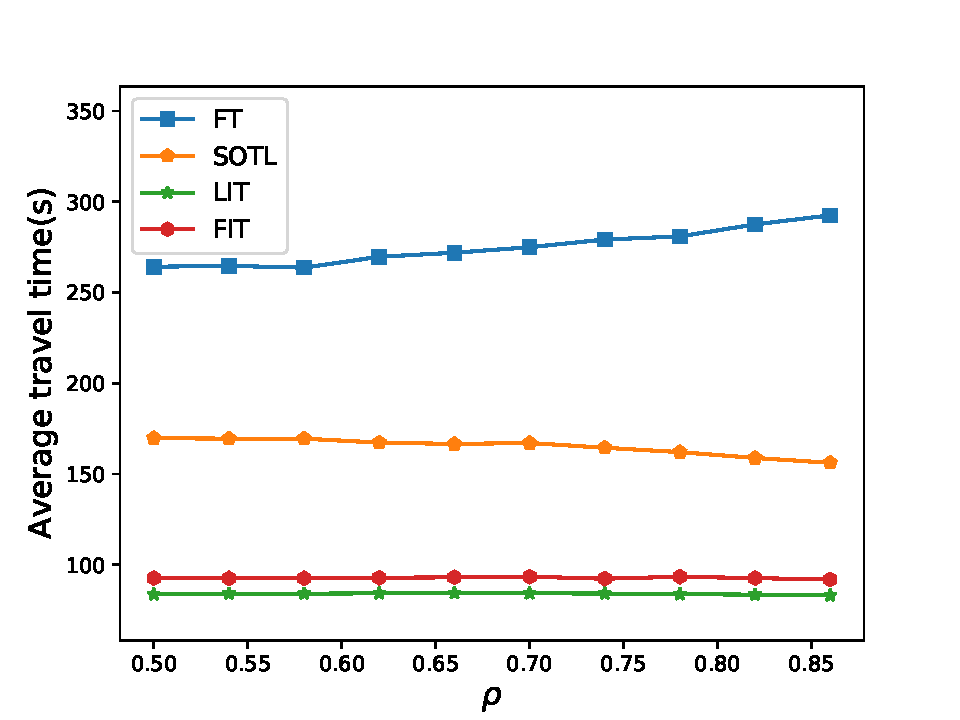
\includegraphics[width=10cm]{fig/efficiency.pdf}
    \caption{效率}
    \label{fig:efficiency}
\end{figure}

其次,由于我们的主要研究目标是公平性,我们首先分析了在使用不同方法下每条车道的延误情况。这里我们用Jain Fairness Index(JFI)来量化公平性指标,JFI的计算方式如下:
\begin{align}
    \mathcal{J}=\frac{\left(\sum_{i=1}^{M} \bar{D}_{i}\right)^{2}}{M \sum_{i=1}^{M} \bar{D}_{i}^{2}},
\end{align}
其中$\bar{D}_{i}$是车道$i$的平均延误时间。当每个车道具有相同的平均延误时间时,JFI的值达到最大值,即1。\autoref{fig:fairness}展示了四种方法在不同$\rho$值下的平均延迟的JFI表现。从中我们可以看出FT和LIT的JFI值随着交通不平衡情况的加剧(即$\rho$值越大)而减小,而FIT任然能偶保持较高的值,并且高于同样能够保持稳定JFI值的SOTL方法。
\begin{figure}[htb]
    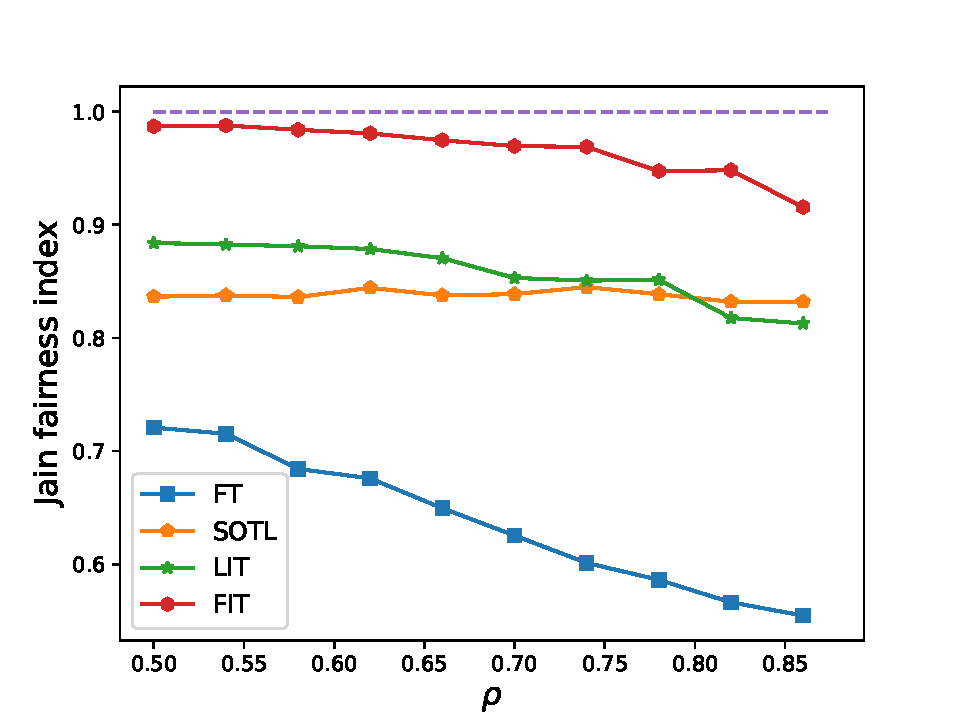
\includegraphics[width=10cm]{fig/fairness.pdf}
    \caption{公平}
    \label{fig:fairness}
\end{figure}

然后,我们更加详细地研究了不同方法的延误情况。下面我们具体分析在主干道和支干道上四种方法在不同的$\rho$值情况下车辆延误时间分布情况。
\begin{figure}[htb]
    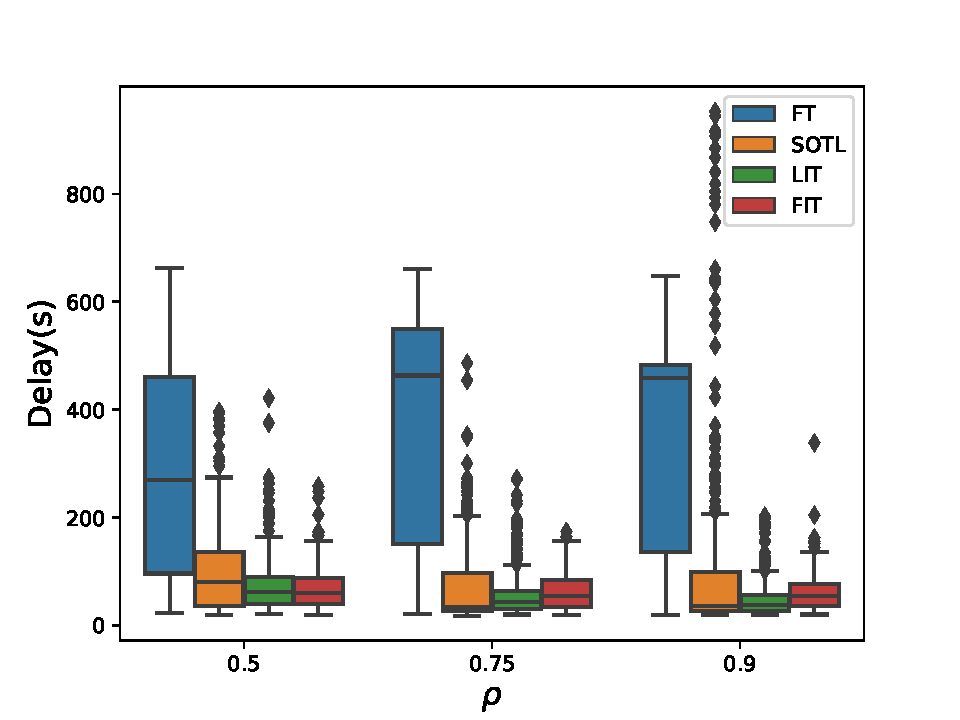
\includegraphics[width=10cm]{fig/major_delay.pdf}
    \caption{主干道(N-S方向)的车辆延误时间分布}
    \label{fig:major_delay}
\end{figure}
从\autoref{fig:major_delay}中我们可以看出,在主干道上,基于学习的方法(LIT和FIT)比传统方法(FT和SOTL)具有更低的延误时间,虽然SOTL方法整体上延迟也比较低,但是会有很多极端值,最高的延误时间甚至超过800$s$。

从\autoref{fig:minor_delay}中我们可以看出,在支干道上,随着$\rho$值的增加(即交通不平衡情况的加重),原先在主干道上表现优异的LIT方法性能开始恶化(),但是FIT依然能够保持一个相对低的延迟。

\begin{figure}[htb]
    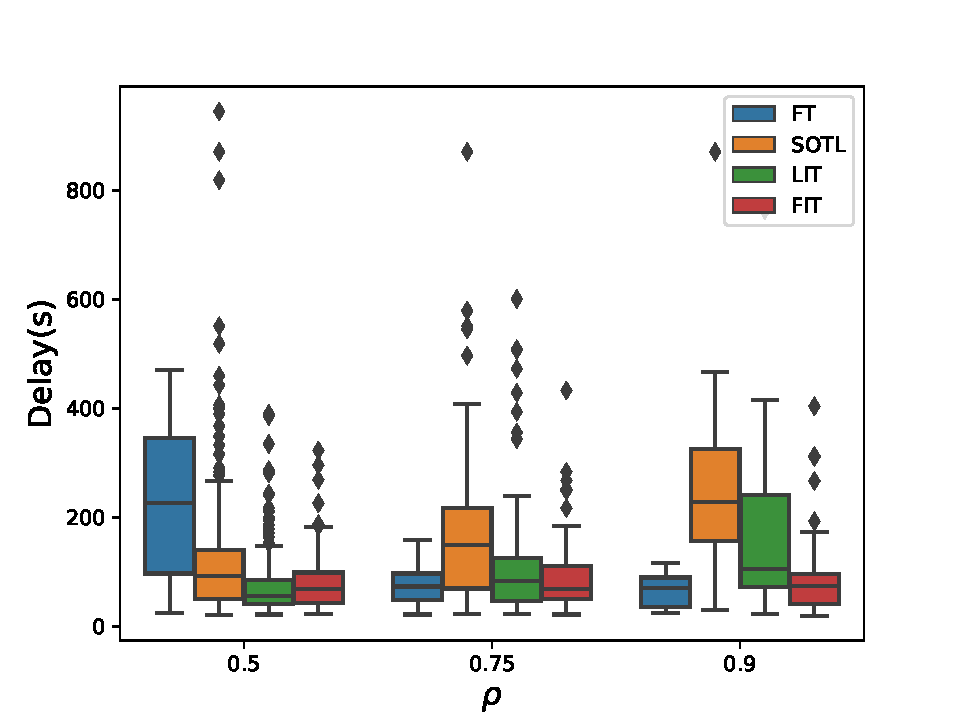
\includegraphics[width=10cm]{fig/minor_delay.pdf}
    \caption{支干道(N-S方向)的车辆延误时间分布}
    \label{fig:minor_delay}
\end{figure}

我们研究了不同方法的驾驶体验得分情况,\autoref{fig:des}展示了在$\rho=0.75$的情况下不同方法的驾驶体验得分分布情况。从中我们可以看出,FT方法超过半数的驾驶体验的分都是1分,由此可以看出该方法的不灵活。对于SOTL方法而言,虽然他的5分的比例最高,但是其得分分布的方差也是最高的。FIT的得分分布与LIT相似,但FIT的方差低于LIT,在以牺牲少量效率为代价的前提下。
\begin{figure}[t]
    \centering
    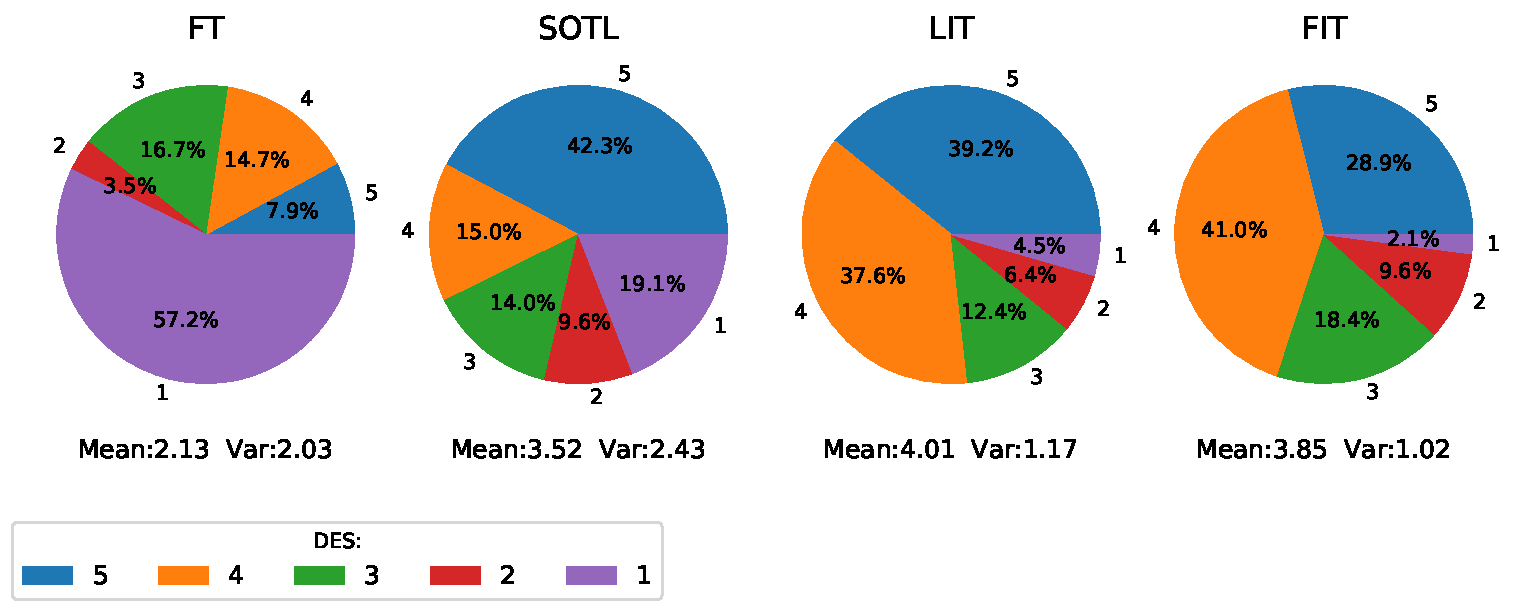
\includegraphics[width=0.9\textwidth]{fig/des.pdf}
    \caption{驾驶体验得分统计}
    \label{fig:des}
\end{figure}

最后,我们研究了$W$参数的影响,因为$W$是用来平衡效率和公平性的,不同的值会导致学习到不同的策略,从\autoref{fig:window-size}中我们可以看出W值越高,越有利于系统的公平性。相反,W值越小,系统效率就越高。具体来说,当$W=1$时,我们方法FIT的整体性能接近于LIT
\begin{figure}[htb]
    
    \subfloat[效率\label{fig:window-size-efficiency}]{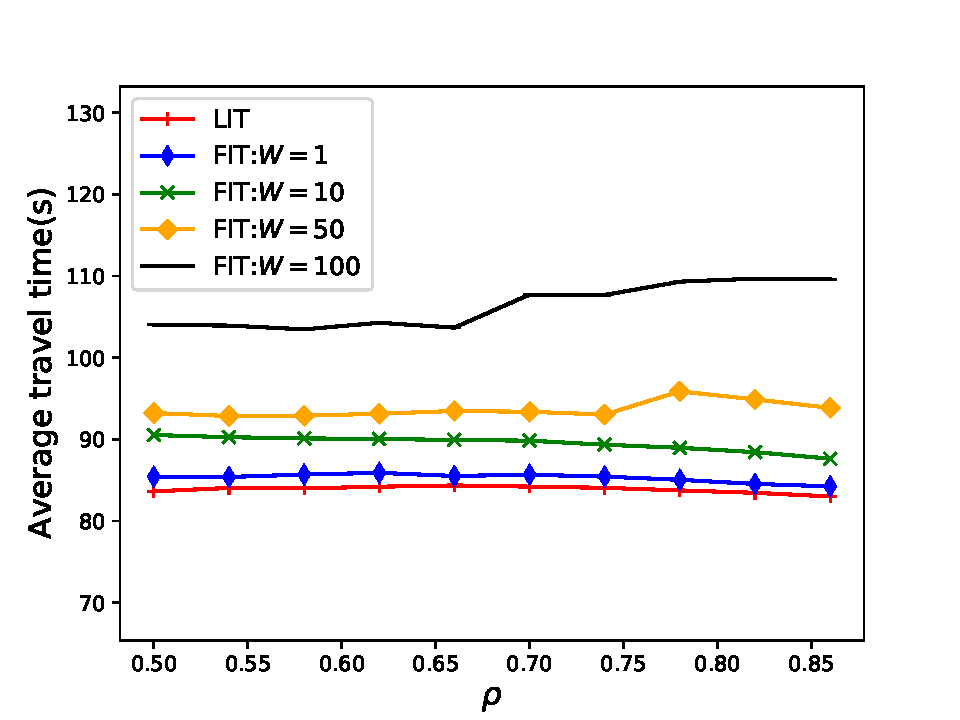
\includegraphics[width=0.4\textwidth]{fig/window_efficiency.pdf}}
    \subfloat[公平性\label{fig:window-size-fairness}]{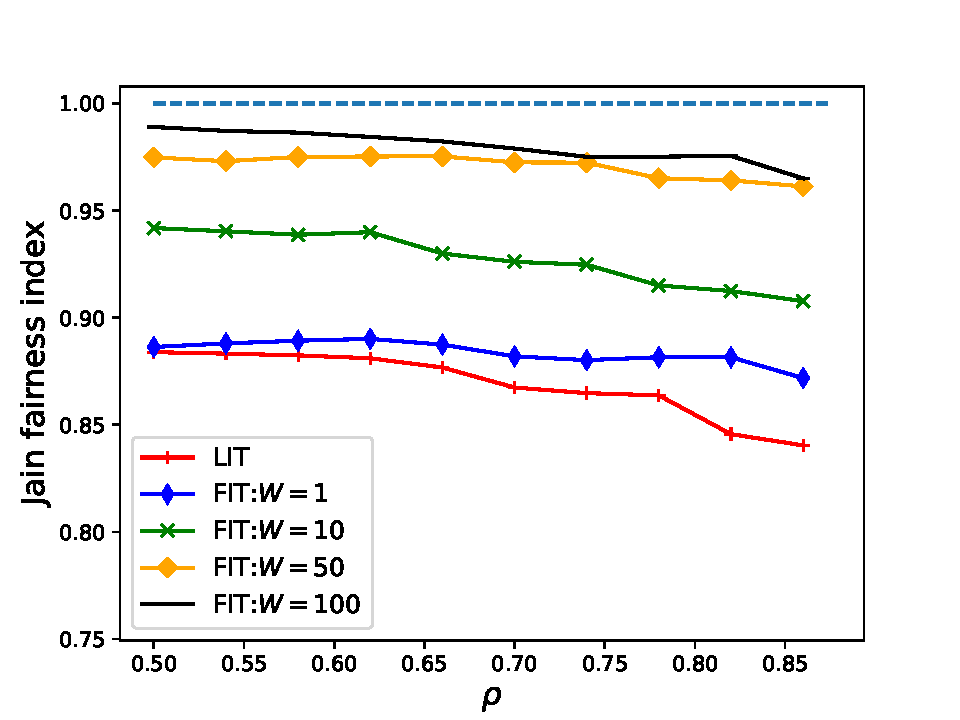
\includegraphics[width=0.4\textwidth]{fig/window_fairness.pdf}}
    \caption{$W$对效率和公平性的影响}
    \label{fig:window-size}
  \end{figure}


